% --- ETUDE DE CAS ---
\newpage
\section*{Étude de cas~: Burnout}
\addcontentsline{toc}{section}{Étude de cas~: Burnout}

\section*{AAV}
\addcontentsline{toc}{section}{AAV}
\begin{itemize}
	\item [1] Citer l'utilité de MVC et MVVM et leurs différences
	\item [1] Décrire le rôle de chaque composant MVC et MVVM
	\item [1] Connaître la syntaxe du langage C\#
	\item [3] Pratiquer le langage C\#
	\item [3] Pratiquer les architectures MVC et MVVM
\end{itemize}

\newpage

\subsection*{Mots clés}
\phantomsection
\addcontentsline{toc}{subsection}{Mots clés}
\begin{itemize}
	\item Modularité
	\item MVC
	\item MVVM
	\item .NET6
	\item C\#
	\item ASP.NET core
	\item Séparation des préoccupations
	\item Principe SOLID
	\item Framework modernes
\end{itemize}

\subsection*{Contexte}
\phantomsection
\addcontentsline{toc}{subsection}{Contexte}
\noindent 2F Roaming souhaite refondre l’architecture de son application afin de réduire les coûts de développement. De plus, la format° des équipes est nécessaire.

\subsection*{Problématique}
\phantomsection
\addcontentsline{toc}{subsection}{Problématique}
\noindent Comment faciliter l’architecture de l’app de l’entreprise afin de réduire les coûts ?

\subsection*{Contraintes}
\phantomsection
\addcontentsline{toc}{subsection}{Contraintes}
\begin{itemize}
	\item Framework imposé
	\item Coûts de dev
	\item Formation équipe
\end{itemize}

\subsection*{Généralisation}
\phantomsection
\addcontentsline{toc}{subsection}{Généralisation}
\begin{itemize}
	\item POO
	\item UML
	\item Framework moderne
	\item Communication technique
\end{itemize}

\subsection*{Livrables}
\phantomsection
\addcontentsline{toc}{subsection}{Livrables}
\begin{itemize}
	\item Nouvelle archi
	\item Plan de formation
\end{itemize}

\subsection*{Pistes de solutions}
\phantomsection
\addcontentsline{toc}{subsection}{Pistes de solutions}
\begin{itemize}
	\item Principes du SOLID
	\item Architecture MVC ou MVVM
	\item Diagramme UML
	\item Séparation des couches
\end{itemize}

\subsection*{Plan d'actions}
\phantomsection
\addcontentsline{toc}{subsection}{Plan d'actions}
\begin{itemize}
	\item Etudier les principes du SOLID
	\item Etudier les diagrammes UML (Séquence, Classe, Cas d'utilisation)
	\item Etudier les types d'architecture (MVC, MVVM)
	\item Proposer une nouvelle architecture
	\begin{itemize}
		\item Réalisation des diagrammes UML
		\item Explication et plan
	\end{itemize}
	\item Documentation des nouvelles pratiques
\end{itemize}

\newpage
\section*{Démarche~: Burnout}
\addcontentsline{toc}{section}{Démarche~: Burnout}


\subsection*{Définition~: Mots clés}
\phantomsection
\addcontentsline{toc}{subsection}{Définition: Mots clés}

\noindent \textbf{Modularité}:
\noindent En informatique et en programmation, la modularité consiste à diviser un système en modules ou composants distincts. Chaque module gère une fonctionnalité spécifique et fonctionne de manière indépendante. Elle simplifie la conception, le développement, les essais et la maintenance en permettant de se concentrer sur une partie à la fois sans affecter le reste du système.

\begin{center}
\rule{5cm}{0.4pt}
\end{center}

\vspace{0.5cm}

\noindent \textbf{MVC (Modèle-Vue-Contrôleur)}:
\noindent MVC (Modèle-Vue-Contrôleur) est un modèle de conception logicielle couramment utilisé pour implémenter les interfaces utilisateurs, les données et la logique de contrôle. Il met l'accent sur la séparation entre la logique métier du logiciel et l'affichage. Cette « séparation des responsabilités » permet une meilleure répartition du travail et une maintenance facilitée. D'autres modèles de conception sont basés sur MVC, comme MVVM (Modèle-Vue-VueModèle), MVP (Modèle-Vue-Présentateur) et MVW (Modèle-Vue-Whatever).

\noindent Les trois parties du modèle de conception logicielle MVC peuvent être décrites ainsi :
\begin{itemize}
	\item \textbf{Modèle} : Gère les données et la logique métier.
    \item \textbf{Vue} : Gère la présentation et l'affichage.
    \item \textbf{Contrôleur} : Transmet les commandes aux parties modèle et vue.
\end{itemize}

\begin{center}
	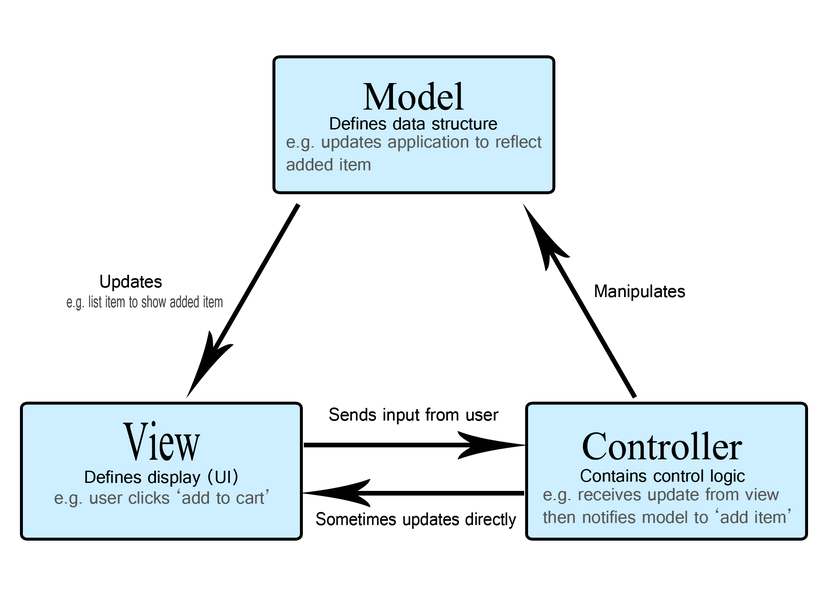
\includegraphics[width=0.8\textwidth]{contents/img/MVC.png}
\end{center}

\newpage

\noindent \textbf{Le Modèle}
\noindent Le modèle définit quelles données l'application doit contenir. Si l'état de ces données change, le modèle notifie généralement la vue (pour que l'affichage soit mis à jour si besoin) et parfois le contrôleur (si une logique différente est nécessaire pour contrôler la vue mise à jour).
\noindent Dans notre application de liste de courses, le modèle spécifierait quelles données doivent être présentes dans chaque élément de la liste — article, prix, etc. — et quels éléments sont déjà présents.

\noindent \textbf{La Vue}
\noindent La vue définit comment les données de l'application doivent être affichées.
\noindent Dans notre application de liste de courses, la vue définirait comment la liste est présentée à l'utilisateur·ice et recevrait les données à afficher depuis le modèle.

\noindent \textbf{Le Contrôleur}
\noindent Le contrôleur contient la logique qui met à jour le modèle et/ou la vue en réponse aux actions des utilisateur·ice·s de l'application.
\noindent Par exemple, notre liste de courses pourrait comporter des formulaires et des boutons permettant d'ajouter ou de supprimer des articles. Ces actions nécessitent la mise à jour du modèle, donc la saisie est envoyée au contrôleur, qui manipule alors le modèle comme il convient, puis envoie les données mises à jour à la vue.

\begin{center}
\rule{5cm}{0.4pt}
\end{center}

\vspace{0.5cm}

\noindent \textbf{C\#}:
\noindent C\# est un langage de programmation orientée objet, fortement typé, dérivé de C et de C++, ressemblant au langage Java. Il est utilisé pour développer des applications web, ainsi que des applications de bureau, des services web, des commandes, des widgets ou des bibliothèques de classes. En C\#, une application est un lot de classes où une des classes comporte une méthode Main, comme cela se fait en Java.

\noindent C\# est destiné à développer sur la plateforme .NET, une pile technologique créée par Microsoft pour succéder à COM.

\noindent Les exécutables en C\# sont subdivisés en assemblies, en namespaces, en classes et en membres de classe. Un assembly est la forme compilée, qui peut être un programme (un exécutable) ou une bibliothèque de classes (une dll). Un assembly contient le code exécutable en CIL, ainsi que les symboles. Le code CIL est traduit en langage machine au moment de l'exécution par la fonction just-in-time de la plateforme .NET. 

\begin{center}
\rule{5cm}{0.4pt}
\end{center}

\vspace{0.5cm}

\noindent \textbf{ASP.NET Core}:
\noindent ASP.NET Core est une infrastructure open source multiplateforme et hautes performances pour la création d’applications web modernes à l’aide de .NET. L’infrastructure est conçue pour le développement d’applications à grande échelle et peut gérer n’importe quelle charge de travail de taille, ce qui en fait un choix robuste pour les applications de niveau entreprise.

\noindent Pourquoi utiliser ASP.NET Core ?
\begin{itemize}
	\item \textbf{Framework unifié} : ASP.NET Core est un framework web complet et entièrement intégré avec des composants intégrés prêts pour la production pour gérer tous vos besoins de développement web.
    \item \textbf{Productivité complète de la pile} : créez plus d’applications plus rapidement en permettant à votre équipe de travailler sur une pile complète, du front-end au serveur principal, à l’aide d’une seule infrastructure de développement.
    \newpage
	\item \textbf{Sécurisé par conception} : ASP.NET Core est conçu avec une sécurité qui constitue une préoccupation majeure et inclut la prise en charge intégrée de l’authentification, de l’autorisation et de la protection des données.
    \item \textbf{Prêt pour le cloud} : que vous déployiez sur vos propres centres de données ou dans le cloud, ASP.NET Core simplifie le déploiement, la supervision et la configuration.
    \item \textbf{Performances et scalabilité} : gérez les charges de travail les plus exigeantes grâce aux performances de pointe d'ASP.NET Core dans le secteur.
    \item \textbf{Fiable et mature} : ASP.NET Core est utilisé et prouvé à hyperscale par certains des plus grands services du monde, notamment Bing, Xbox, Microsoft 365 et Azure.
\end{itemize}

\begin{center}
\rule{5cm}{0.4pt}
\end{center}

\vspace{0.5cm}

\noindent \textbf{Séparation des préoccupations}:
\noindent La séparation des préoccupations (SoC) est un principe de conception logiciel qui consiste à diviser un programme informatique en sections distinctes, chacune traitant d'une préoccupation spécifique ou d'un aspect particulier du programme. L'objectif principal de la SoC est de réduire la complexité du code, d'améliorer la maintenabilité et de faciliter la réutilisation des composants.

\begin{center}
\rule{5cm}{0.4pt}
\end{center}

\vspace{0.5cm}

\noindent \textbf{Principe SOLID}:
\noindent Les principes SOLID consistent en cinq pratiques et directives pour un code propre, maintenable et flexible lors de la programmation orientée objet (OOP).

\begin{itemize}
	\item \textbf{Single Responsibility Principle} ou Principe de Responsabilité Unique : une classe ne doit avoir qu’une seule responsabilité (et non une seule tâche) et une seule raison de changer.
	\item \textbf{Open Closed Principle} ou Principe d’Ouverture/Fermeture : les classes doivent être ouvertes aux extensions et fermées aux modifications.
	\item \textbf{Liskov Substitution Principle} ou Principe de Substitution de Liskov : les sous-classes doivent pouvoir hériter et implémenter toutes les méthodes et propriétés de la superclasse.
	\item \textbf{Interface Segregation Principle} ou Principe de Ségrégation des interfaces : les interfaces ne doivent pas contenir plus de méthodes qu’il n’en faut pour les classes qui les implémentent.
	\item \textbf{Dependency Inversion Principle} ou Principe d’Inversion de Dépendance : les classes ne doivent pas dépendre d’autres classes, mais d’interfaces ou de classes abstraites.
\end{itemize}

\newpage

Les avantages de l’application des SOLID Principles permettent que le code soit :
\begin{itemize}
	\item \textbf{Clair, propre et beau} : les logiciels et les codes sont plus faciles à comprendre, plus compréhensibles, plus efficaces et tout simplement plus beaux.
	\item \textbf{Facile à entretenir} : grâce à une structure claire et concise, il est plus facile d’entretenir et de maintenir le code, qu’il soit nouveau ou qu’il ait évolué au fil du temps, même si plusieurs personnes sont impliquées.
	\item \textbf{Adaptable, extensible, réutilisable} : grâce à une meilleure lisibilité, à une réduction des complexités et des responsabilités ainsi qu’à une réduction des dépendances entre les classes, le code peut être plus facilement édité, adapté, étendu par des interfaces et réutilisé de manière flexible.
	\item \textbf{Moins sujet aux erreurs} : avec un code propre et une structure simple, les modifications apportées à une partie n’ont pas d’impact involontaire sur d’autres domaines ou fonctions.
	\item \textbf{Plus sûr et plus fiable} : en réduisant ou en éliminant les points faibles, les incompatibilités ou les erreurs, on améliore la fonctionnalité et la fiabilité des systèmes, et donc la sécurité.
\end{itemize}

\begin{center}
\rule{5cm}{0.4pt}
\end{center}

\vspace{0.5cm}

\noindent \textbf{Framework modernes}:
\noindent  Un framework est un ensemble de composants logiciels réutilisables qui permettent de développer de nouvelles applications plus efficacement. Il fournit une structure de base et des fonctionnalités prêtes à l'emploi, ce qui permet aux développeurs de se concentrer sur la logique métier spécifique de leur application plutôt que de réinventer la roue à chaque fois.	

\begin{itemize}
	\item \textbf{Améliorer la qualité du code} : Les frameworks logiciels contiennent des composants logiciels conçus selon des normes de programmation élevées. Les développeurs peuvent utiliser le framework logiciel avec la certitude que moins de bogues affecteront les codes sous-jacents
	\item \textbf{Gagner du temps sur le développement} : Les frameworks logiciels améliorent l'efficacité de la programmation et les entreprises peuvent les utiliser pour publier des applications fonctionnelles plus rapidement. Avec un bon framework logiciel, les développeurs peuvent se concentrer sur l'écriture de code de haut niveau qui gère la logique métier plutôt que sur des modules de codage de base.
	\item \textbf{Meilleure sécurité logicielle} : Avec une base de code élargie, il est difficile pour les développeurs de détecter les problèmes de sécurité du code et d'y répondre. En revanche, un bon framework logiciel comprend des points de contrôle de sécurité prêts à l'emploi qui permettent aux développeurs de renforcer plus facilement la sécurité du code et des données.
	\item \textbf{Révision efficace du code} : En utilisant un framework, les équipes logicielles peuvent valider leurs applications à l'aide de scénarios de test complets et d'une couverture de code. De plus, les développeurs trouvent qu'il est plus facile de déboguer et de corriger les problèmes de code dans un framework bien structuré.
	\newpage
	\item \textbf{Flexibilité de développement} : Ils peuvent retenir le code spécifique au projet tout en échangeant différents frameworks adaptés à leurs objectifs. Cela réduit les réécritures de code que les développeurs doivent effectuer.
\end{itemize}

\begin{center}
\rule{5cm}{0.4pt}
\end{center}

\vspace{0.5cm}

\noindent \textbf{MVVM}:
\noindent Le modèle MVVM (Modèle-Vues-Vues-Modèle) permet de séparer de manière nette la logique métier et la logique de présentation d’une application de son interface utilisateur (IU). Le maintien d’une séparation nette entre la logique d’application et l’IU permet de résoudre de nombreux problèmes de développement et de faciliter le test, la maintenance ainsi que l’évolution d’une application. Il permet également d’améliorer considérablement les opportunités de réutilisation du code.

\noindent Il existe trois composants principaux dans le modèle MVVM : le modèle, la vue et le modèle de vue. Chacun sert un objectif distinct. Le diagramme ci-dessous montre les relations entre les trois composants

\vspace{0.5cm}

\begin{center}
	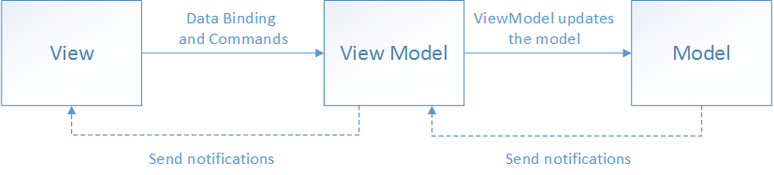
\includegraphics[width=\textwidth]{contents/img/MVVM.png}
\end{center}

\begin{center}
\rule{5cm}{0.4pt}
\end{center}

\vspace{0.5cm}

\noindent \textbf{.NET6}:
\noindent .NET 6 est une plateforme de développement open source, multiplateforme et hautes performances créée par Microsoft. Elle permet aux développeurs de créer une variété d'applications, notamment des applications web, des applications de bureau, des services cloud, des applications mobiles et des applications IoT (Internet des objets).

\newpage

\section*{Workshop}
\addcontentsline{toc}{section}{Workshop}

\subsection*{Qu’est-ce qu’un diagramme UML ?}
\phantomsection
\addcontentsline{toc}{subsection}{Qu’est-ce qu’un diagramme UML ?}
Les diagrammes UML sont la représentation de la notation UML. Elle se compose d’éléments standardisés (tels que des composants, des classes et des cas d’utilisation) qui sont connectés à l’aide de relations (flèches) pour représenter l’architecture, l’implé-mentation et la structure d’un système logiciel par ailleurs complexe.

\vspace{0.5cm}

\begin{center}
	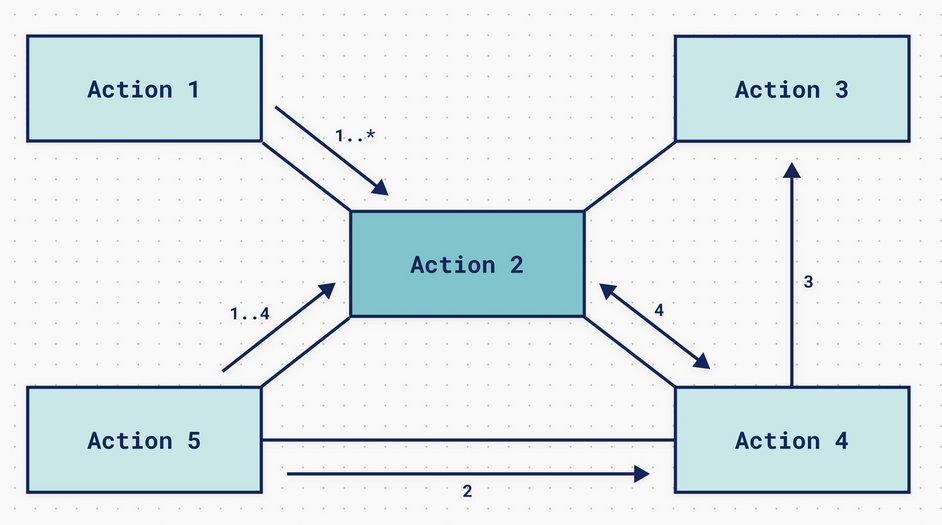
\includegraphics[width=0.8\textwidth]{contents/img/UML.png}
\end{center}

\vspace{0.5cm}

\noindent Les diagrammes UML représentent le plus souvent les éléments suivants :

\begin{itemize}
	\item Les composants du système et comment ils interagissent avec les autres
    \item L’interface utilisateur du système
    \item Les activités ou travaux effectués par les composants ou les interfaces
    \item Comment différentes entités interagissent avec les composants et les interfaces
    \item La manière dont le système fonctionne
\end{itemize}

\noindent Le modèle UML est composé d’une combinaison de diagrammes. Les 14 types de diagrammes UML représentent le modèle de manière structurelle ou comportementale, comme vous pouvez le voir ci-dessous.

\newpage

\subsection*{Diagrammes UML structurels}
\phantomsection
\addcontentsline{toc}{subsection}{Diagrammes UML structurels}
Les diagrammes structurels UML représentent la structure statique d’un système. Ces diagrammes utilisent des objets, des opérations, des relations et des attributs pour analyser ou décrire cette structure. Sous les diagrammes UML structurels se trouvent les types suivants :

\vspace{0.5cm}

\begin{itemize}
	\item Diagramme de classes
	\item Diagramme de composants
	\item Diagramme de déploiement
	\item Diagramme d’objets
	\item Diagramme de packages
	\item Diagramme de structure composite
	\item Diagramme de profils
\end{itemize}

\begin{center}
	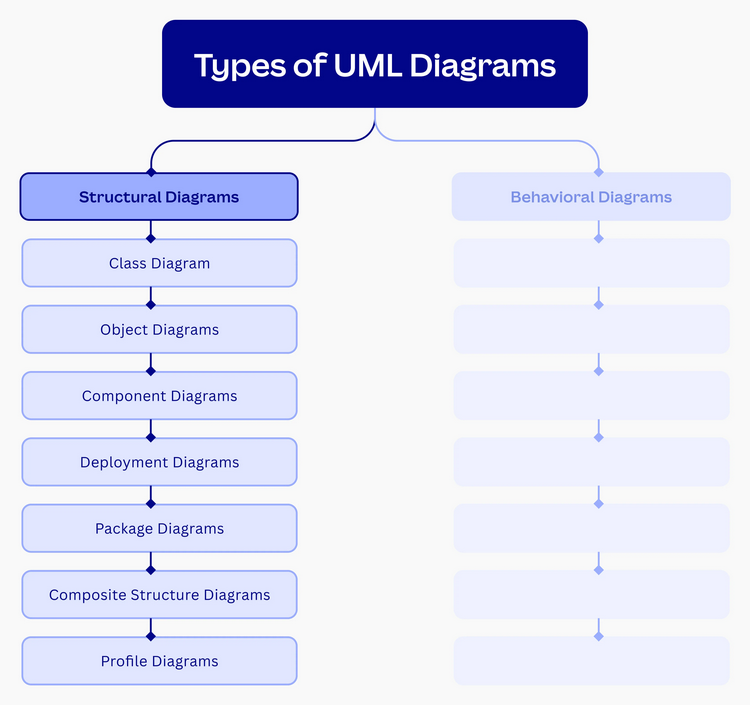
\includegraphics[width=0.8\textwidth]{contents/img/diagram_UML.png}
\end{center}

\subsection*{Diagrammes de classe}
\phantomsection
\addcontentsline{toc}{subsection}{Diagrammes de classe}
Un diagramme de classe UML est généralement utilisé pour visualiser les composants d’un système dans la programmation orientée objet. Il représente les classes (avec leur visibilité, leurs portées, leurs signaux, leurs types de données, leurs packages, leurs interfaces et leurs objets) et leurs relations. Pour une vue plus détaillée, ces classes peuvent également être divisées en sous-classes.

\noindent Généralement utilisés pour la modélisation conceptuelle d’une application, les diagrammes de classe UML peuvent également être facilement traduits en code de programmation et sont aussi utilisés dans la modélisation de données.

\noindent Par principe, les diagrammes de classe UML sont représentés à l’aide des éléments suivants :

\begin{itemize}
	\item \textbf{Classes} : ce composant est constitué d’un rectangle où le nom de la classe (sa première lettre en majuscule) est récrit en gras et au milieu. Les attributs (valeurs qui détaillent une instance de classe) sont alignés à gauche avec les premières lettres en minuscules. Pour finir, les opérations, ou les actions que la classe peut exécuter, sont alignées à gauche avec les premières lettres en minuscules.
	\item \textbf{Relations entre classes} : représentées par un trait en pointillés ou plein selon le type de relation (association, héritage, réalisation, dépendance, agrégation ou composition).
\end{itemize}

\vspace{0.5cm}

\begin{center}
	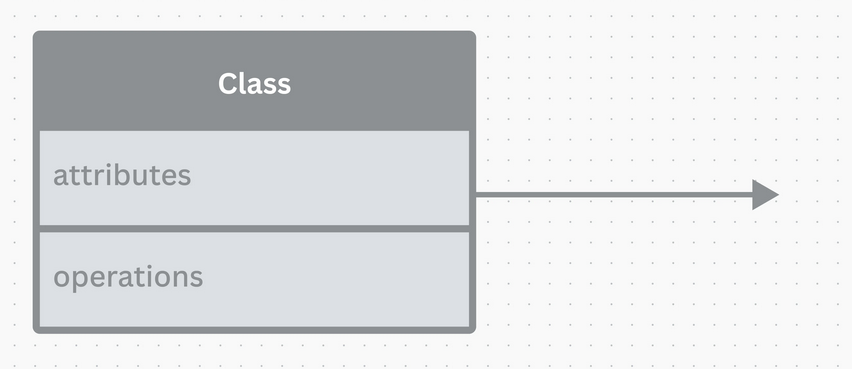
\includegraphics[width=0.8\textwidth]{contents/img/diagram_class.png}
\end{center}

\newpage

\subsection*{Diagrammes de séquençage}
\phantomsection
\addcontentsline{toc}{subsection}{Diagrammes de séquençage}
Un diagramme de séquence UML affiche la séquence requise pour exécuter une fonctionnalité. Il représente les processus et les objets impliqués dans la fonctionnalité et la séquence de messages échangés entre eux.

\noindent Les diagrammes de séquence, ou diagrammes d’événements, sont généralement utilisés en génie logiciel pour capturer la manière dont les opérations sont effectuées et la manière dont le codage logiciel peut être effectué pour réaliser la séquence de cas d’utilisation.

\noindent Les diagrammes de séquence UML sont représentés comme suit :
\begin{itemize}
	\item \textbf{Acteur} : un bonhomme bâton.
	\item \textbf{Participant individuel à l’interaction} : une ligne pointillée avec un rectangle en haut.
	\item \textbf{Temps entre le début et la fin de l’interaction} : représenté par un rectangle avec une bordure fine sur la ligne de vie.
	\item \textbf{Message entre deux lignes de vie} : texte à côté d’une flèche indiquant la direction du message.
	\item \textbf{Remarques sur les éléments} : annotations.
\end{itemize}

\vspace{0.5cm}

\begin{center}
	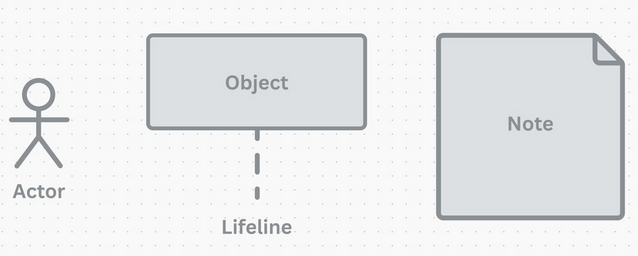
\includegraphics[width=0.8\textwidth]{contents/img/diagram_sequence.png}
\end{center}

\newpage

\subsection*{Diagrammes de cas d'utilisation}
\phantomsection
\addcontentsline{toc}{subsection}{Diagrammes de cas d'utilisation}
Un diagramme de cas d’utilisation UML, comme son nom l’indique, décrit le cas d’utilisation d’un système. Autrement dit, il affiche les interactions possibles qu’un utilisateur peut avoir avec un système et permet de présenter le système du point de vue de l’utilisateur final.

\noindent Les diagrammes de cas d’utilisation sont utilisés dans les pratiques de développement de logiciels, d’entreprise ou de modélisation commerciale pour offrir aux parties prenantes non techniques une vue d’ensemble du système. Ils permettent de comprendre la manière dont le système sera conçu.

\noindent Les diagrammes de cas d’utilisation UML sont représentés comme suit :
\begin{itemize}
	\item \textbf{Acteur} : le participant qui interagit avec le système, représenté sous la forme d’un bonhomme bâton.
	\item \textbf{Cas d’utilisation} : une fonction système automatisée ou manuelle décrite par un verbe et représentée par une ellipse. Les cas d’utilisation doivent être associés à des acteurs.
	\item \textbf{Lien de communication} : utilisé pour montrer l’association entre les acteurs et les cas d’utilisation. Il est représenté par des flèches.
	\item \textbf{Limite du système} : représenté sous forme de rectangles. Les acteurs et les cas d’utilisation entrent dans ce cadre.
\end{itemize}

\vspace{0.5cm}

\begin{center}
	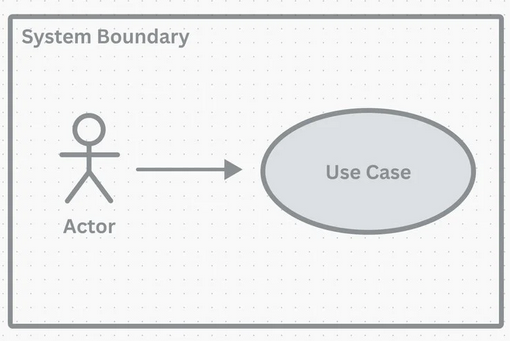
\includegraphics[width=0.6\textwidth]{contents/img/diagram_usecase.png}
\end{center}

\newpage

\subsection*{Diagrammes d'activité}
\phantomsection
\addcontentsline{toc}{subsection}{Diagrammes d'activité}
Un diagramme d’activité UML décrit les activités, les actions et les flux de travail des processus informatiques ou organisationnels. Il s’agit essentiellement d’un logigramme avancé qui modélise le flux des opérations d’un système ou d’une organisation.

\noindent Les diagrammes d’activité sont généralement utilisés dans le design de systèmes embarqués pour visualiser la relation entre les cas d’utilisation et les processus métier.

\noindent Les diagrammes d’activités UML sont représentés comme suit :
\begin{itemize}
	\item \textbf{Actions} : rectangles arrondis
	\item \textbf{Décisions} : losanges
	\item \textbf{Activités simultanées} : barres
	\item \textbf{Début du processus} : cercle noir
	\item \textbf{Arrêt du processus} : cercle noir avec bordure
\end{itemize}

\vspace{0.5cm}

\begin{center}
	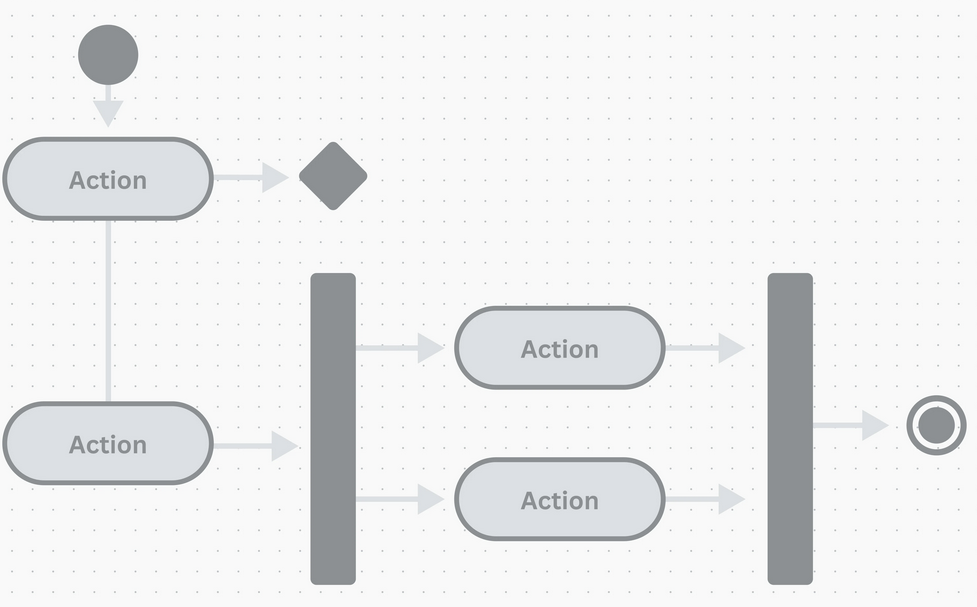
\includegraphics[width=0.8\textwidth]{contents/img/diagram_activite.png}
\end{center}

\newpage

\subsection*{Diagrammes d'objets}
\phantomsection
\addcontentsline{toc}{subsection}{Diagrammes d'objets}
Un diagramme d’objet UML est une instance d’un diagramme de classe où des exemples réels sont utilisés pour représenter le système. Il représente les objets et les relations entre eux, ce qui peut être utile pour créer des diagrammes de classe ou pour vérifier l’exactitude et l’exhaustivité d’un diagramme. Les diagrammes d’objet sont également largement utilisés dans la programmation orientée objet.

\noindent Tout comme les diagrammes de classe, les diagrammes d’objets sont également représentés comme suit :
\begin{itemize}
	\item \textbf{Objet} : un rectangle avec le nom de l’objet, séparé par deux points de sa classe et souligné, et les attributs de l’objet. Contrairement aux classes, les attributs d’objet doivent se voir attribuer des valeurs.
	\item \textbf{Relations entre objets} : des lignes qui dénotent une association, un héritage, une réalisation, une dépendance, une agrégation ou une composition.
\end{itemize}

\vspace{0.5cm}

\begin{center}
	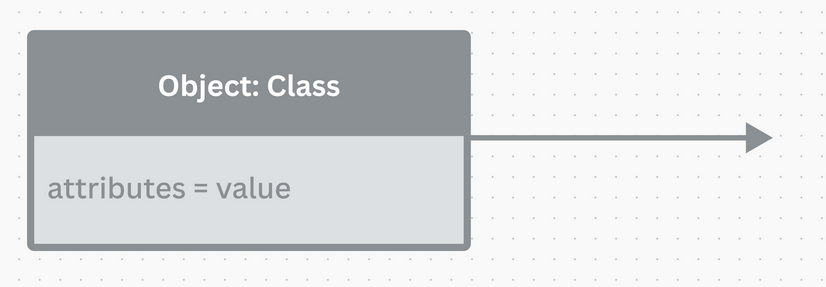
\includegraphics[width=0.8\textwidth]{contents/img/diagram_object.png}
\end{center}

\vspace{0.5cm}

\subsection*{Pourquoi utiliser l’UML en POO ?}
\phantomsection
\addcontentsline{toc}{subsection}{Pourquoi utiliser l’UML en POO ?}
\noindent En POO, on manipule des concepts abstraits (classes, héritage, interfaces). Sans schéma, on se perd vite dans la complexité. L'UML permet de :

\begin{itemize}
	\item Communiquer entre développeurs (et avec les clients).
	\item Anticiper les erreurs de conception avant d'écrire la moindre ligne de code.
	\item Générer automatiquement du squelette de code.
\end{itemize}

\newpage

\section*{Analyse et résolution : Burnout}
\addcontentsline{toc}{section}{Analyse et résolution : Burnout}

\subsection*{Conclusion}
\phantomsection
\addcontentsline{toc}{subsection}{Conclusion}

\newpage

\section*{Capitalisation}
\addcontentsline{toc}{section}{Capitalisation}

\begin{center}
\setlength{\tabcolsep}{10pt}

\begin{tabular}{|p{0.30\textwidth}|p{0.45\textwidth}|m{0.08\textwidth}|}
\hline
\textbf{AAV} & \textbf{Commentaire} & \textbf{Statut} \\ \hline

Citer l'utilité de MVC et MVVM et leurs différences &
Les concepts de MVC et MVVM sont expliqués, différences et utilités bien identifiées, exemples et schémas fournis. &
{\color{green!60!black}Acquis} \\ \hline

Décrire le rôle de chaque composant MVC et MVVM &
Rôles du Modèle, Vue, Contrôleur et Modèle de Vue explicités, avec illustrations et explications claires. &
{\color{green!60!black}Acquis} \\ \hline

Connaître la syntaxe du langage C\# &
Principes de base, structure, types, classes et méthodes C\# présentés avec exemples. &
{\color{green!60!black}Acquis} \\ \hline

Pratiquer le langage C\# &
Exercices et exemples pratiques de code C\# réalisés, manipulation des concepts fondamentaux. &
{\color{green!60!black}Acquis} \\ \hline

Pratiquer les architectures MVC et MVVM &
Mise en œuvre concrète des architectures MVC et MVVM dans des exemples ou mini-projets. &
{\color{green!60!black}Acquis} \\ \hline

\end{tabular}
\end{center}

\section*{Ressources}
\addcontentsline{toc}{section}{Ressources}

\begin{itemize}
	\item \textbf{Documentation officielle de Git} : \url{https://git-scm.com/doc}
	\item \textbf{Pro Git Book} : \url{https://git-scm.com/book/en/v2}
	\item \textbf{GitHub Learning Lab} : \url{https://lab.github.com/}
	\item \textbf{POO} : \url{https://docs.microsoft.com/fr-fr/dotnet/csharp/fundamentals/object-oriented/}
	\item \textbf{C\# Guide} : \url{https://docs.microsoft.com/fr-fr/dotnet/csharp/}
	\item \textbf{LINQ} : \url{https://docs.microsoft.com/fr-fr/dotnet/csharp/programming-guide/concepts/linq/}
	\item \textbf{Async/Await} : \url{https://docs.microsoft.com/fr-fr/dotnet/csharp/programming-guide/concepts/async/}
\end{itemize}
